\documentclass{standalone}

\usepackage{tikz}
\usetikzlibrary{shapes.geometric}
\usetikzlibrary{arrows.meta}

\newcommand{\drawHouse}[2]{ % #1: position, #2: scale
    \node[scale=#2] at (#1) {
        
\begin{tikzpicture}[baseline=(house.south), scale=0.15]
            \coordinate (roof_peak) at (0,1);
            \coordinate (roof_left) at (-0.7,0.5);
            \coordinate (roof_right) at (0.7,0.5);
            \coordinate (house_top_left) at (-0.7,0.5);
            \coordinate (house_top_right) at (0.7,0.5);
            \coordinate (house_bottom_left) at (-0.7,-0.5);
            \coordinate (house_bottom_right) at (0.7,-0.5);

            \fill[orange!90!black] (roof_left) -- (roof_peak) -- (roof_right) -- cycle;
            \fill[orange!70!black] (house_top_left) rectangle (house_bottom_right);

            % Door/Boxes
            \draw[fill=white!80!black] (-0.3, -0.5) rectangle (0.3, 0);
            \foreach \i in {0, 0.2, 0.4} {
                \draw[fill=white!80!black] (0.4, -0.4 + \i) rectangle (0.6, -0.2 + \i);
            }
            \node[inner sep=0pt, minimum size=0pt] (house) at (0,-0.5) {}; % for baseline
        \end{tikzpicture}
    };
}

\newcommand{\drawCar}[2]{ % #1: position, #2: scale
    \node[scale=#2] at (#1) {
        
\begin{tikzpicture}[scale=0.15, baseline=(car.south)]
            % Body of the car
            \fill[orange!90!black] (-0.8, 0) rectangle (0.8, 0.5);
            % Cabin
            \fill[orange!90!black] (-0.4, 0.5) rectangle (0.4, 0.8);

            % Wheels
            \fill[gray!70!black] (-0.5, 0) circle (0.15);
            \fill[gray!70!black] (0.5, 0) circle (0.15);
            \node[inner sep=0pt, minimum size=0pt] (car) at (0,0) {}; % for baseline
        \end{tikzpicture}
    };
}


\begin{document}
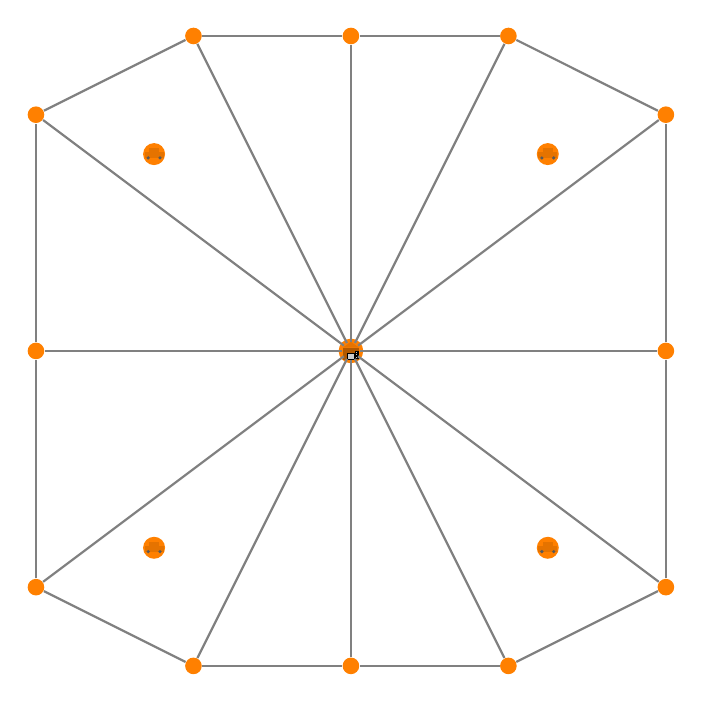
\begin{tikzpicture}[
    node distance=2cm,
    every node/.style={fill=orange, circle, minimum size=6pt, inner sep=0pt},
    line style/.style={gray, thick}
]

    % Warehouse in the center
    \node (center_house) at (0,0) {};
    \drawHouse{0,0}{1}; % Draw the house at (0,0) with scale 1

    % Define outer nodes
    \node (n1) at (-4, 3) {};
    \node (n2) at (-2, 4) {};
    \node (n3) at (0, 4) {};
    \node (n4) at (2, 4) {};
    \node (n5) at (4, 3) {};
    \node (n6) at (4, 0) {};
    \node (n7) at (4, -3) {};
    \node (n8) at (2, -4) {};
    \node (n9) at (0, -4) {};
    \node (n10) at (-2, -4) {};
    \node (n11) at (-4, -3) {};
    \node (n12) at (-4, 0) {};

    % Draw lines from center to outer nodes
    \foreach \n in {n1, n2, n3, n4, n5, n6, n7, n8, n9, n10, n11, n12} {
        \draw[line style] (center_house) -- (\n);
    }

    % Draw routes connecting outer nodes
    \draw[line style] (n1) -- (n2);
    \draw[line style] (n2) -- (n3);
    \draw[line style] (n3) -- (n4); % Adjusted for better flow as per image
    \draw[line style] (n4) -- (n5);
    \draw[line style] (n5) -- (n6);
    \draw[line style] (n6) -- (n7);
    \draw[line style] (n7) -- (n8);
    \draw[line style] (n8) -- (n9);
    \draw[line style] (n9) -- (n10);
    \draw[line style] (n10) -- (n11);
    \draw[line style] (n11) -- (n12);
    \draw[line style] (n12) -- (n1);

    % Draw cars
    \drawCar{-2.5, 2.5}{1}; % Car on the top-left route
    \drawCar{2.5, 2.5}{1};  % Car on the top-right route
    \drawCar{-2.5, -2.5}{1}; % Car on the bottom-left route
    \drawCar{2.5, -2.5}{1}; % Car on the bottom-right route

\end{tikzpicture}
\end{document}